\documentclass[man]{apa6}
\usepackage{lmodern}
\usepackage{amssymb,amsmath}
\usepackage{ifxetex,ifluatex}
\usepackage{fixltx2e} % provides \textsubscript
\ifnum 0\ifxetex 1\fi\ifluatex 1\fi=0 % if pdftex
  \usepackage[T1]{fontenc}
  \usepackage[utf8]{inputenc}
\else % if luatex or xelatex
  \ifxetex
    \usepackage{mathspec}
  \else
    \usepackage{fontspec}
  \fi
  \defaultfontfeatures{Ligatures=TeX,Scale=MatchLowercase}
\fi
% use upquote if available, for straight quotes in verbatim environments
\IfFileExists{upquote.sty}{\usepackage{upquote}}{}
% use microtype if available
\IfFileExists{microtype.sty}{%
\usepackage{microtype}
\UseMicrotypeSet[protrusion]{basicmath} % disable protrusion for tt fonts
}{}
\usepackage{hyperref}
\hypersetup{unicode=true,
            pdftitle={An Attempt at Collaboration with GitKraken},
            pdfauthor={Akhila Nekkanti, Kyle Reardon, Brock Rowley, \& Jeff Gau},
            pdfkeywords={add, some, keywords, words, keys, Yo, Key, Word},
            pdfborder={0 0 0},
            breaklinks=true}
\urlstyle{same}  % don't use monospace font for urls
\usepackage{graphicx,grffile}
\makeatletter
\def\maxwidth{\ifdim\Gin@nat@width>\linewidth\linewidth\else\Gin@nat@width\fi}
\def\maxheight{\ifdim\Gin@nat@height>\textheight\textheight\else\Gin@nat@height\fi}
\makeatother
% Scale images if necessary, so that they will not overflow the page
% margins by default, and it is still possible to overwrite the defaults
% using explicit options in \includegraphics[width, height, ...]{}
\setkeys{Gin}{width=\maxwidth,height=\maxheight,keepaspectratio}
\IfFileExists{parskip.sty}{%
\usepackage{parskip}
}{% else
\setlength{\parindent}{0pt}
\setlength{\parskip}{6pt plus 2pt minus 1pt}
}
\setlength{\emergencystretch}{3em}  % prevent overfull lines
\providecommand{\tightlist}{%
  \setlength{\itemsep}{0pt}\setlength{\parskip}{0pt}}
\setcounter{secnumdepth}{0}
% Redefines (sub)paragraphs to behave more like sections
\ifx\paragraph\undefined\else
\let\oldparagraph\paragraph
\renewcommand{\paragraph}[1]{\oldparagraph{#1}\mbox{}}
\fi
\ifx\subparagraph\undefined\else
\let\oldsubparagraph\subparagraph
\renewcommand{\subparagraph}[1]{\oldsubparagraph{#1}\mbox{}}
\fi

%%% Use protect on footnotes to avoid problems with footnotes in titles
\let\rmarkdownfootnote\footnote%
\def\footnote{\protect\rmarkdownfootnote}


  \title{An Attempt at Collaboration with GitKraken}
    \author{Akhila Nekkanti\textsuperscript{1}, Kyle Reardon\textsuperscript{1},
Brock Rowley\textsuperscript{1}, \& Jeff Gau\textsuperscript{1}}
    \date{}
  
\shorttitle{Lab 8}
\affiliation{
\vspace{0.5cm}
\textsuperscript{1} University of Oregon}
\keywords{add, some, keywords, words, keys, Yo, Key, Word}
\usepackage{csquotes}
\usepackage{upgreek}
\captionsetup{font=singlespacing,justification=justified}

\usepackage{longtable}
\usepackage{lscape}
\usepackage{multirow}
\usepackage{tabularx}
\usepackage[flushleft]{threeparttable}
\usepackage{threeparttablex}

\newenvironment{lltable}{\begin{landscape}\begin{center}\begin{ThreePartTable}}{\end{ThreePartTable}\end{center}\end{landscape}}

\makeatletter
\newcommand\LastLTentrywidth{1em}
\newlength\longtablewidth
\setlength{\longtablewidth}{1in}
\newcommand{\getlongtablewidth}{\begingroup \ifcsname LT@\roman{LT@tables}\endcsname \global\longtablewidth=0pt \renewcommand{\LT@entry}[2]{\global\advance\longtablewidth by ##2\relax\gdef\LastLTentrywidth{##2}}\@nameuse{LT@\roman{LT@tables}} \fi \endgroup}


\DeclareDelayedFloatFlavor{ThreePartTable}{table}
\DeclareDelayedFloatFlavor{lltable}{table}
\DeclareDelayedFloatFlavor*{longtable}{table}
\makeatletter
\renewcommand{\efloat@iwrite}[1]{\immediate\expandafter\protected@write\csname efloat@post#1\endcsname{}}
\makeatother

\authornote{

Correspondence concerning this article should be addressed to Akhila
Nekkanti, Center for Translational Neuroscience University of Oregon
1585 E 13th Ave. Eugene, OR 97403. E-mail:
\href{mailto:akhilan@uoregon.edu}{\nolinkurl{akhilan@uoregon.edu}}}

\abstract{
This is our abstract and it's really something else! SO abstract! And so
concise!


}

\begin{document}
\maketitle

\begin{figure}
\centering
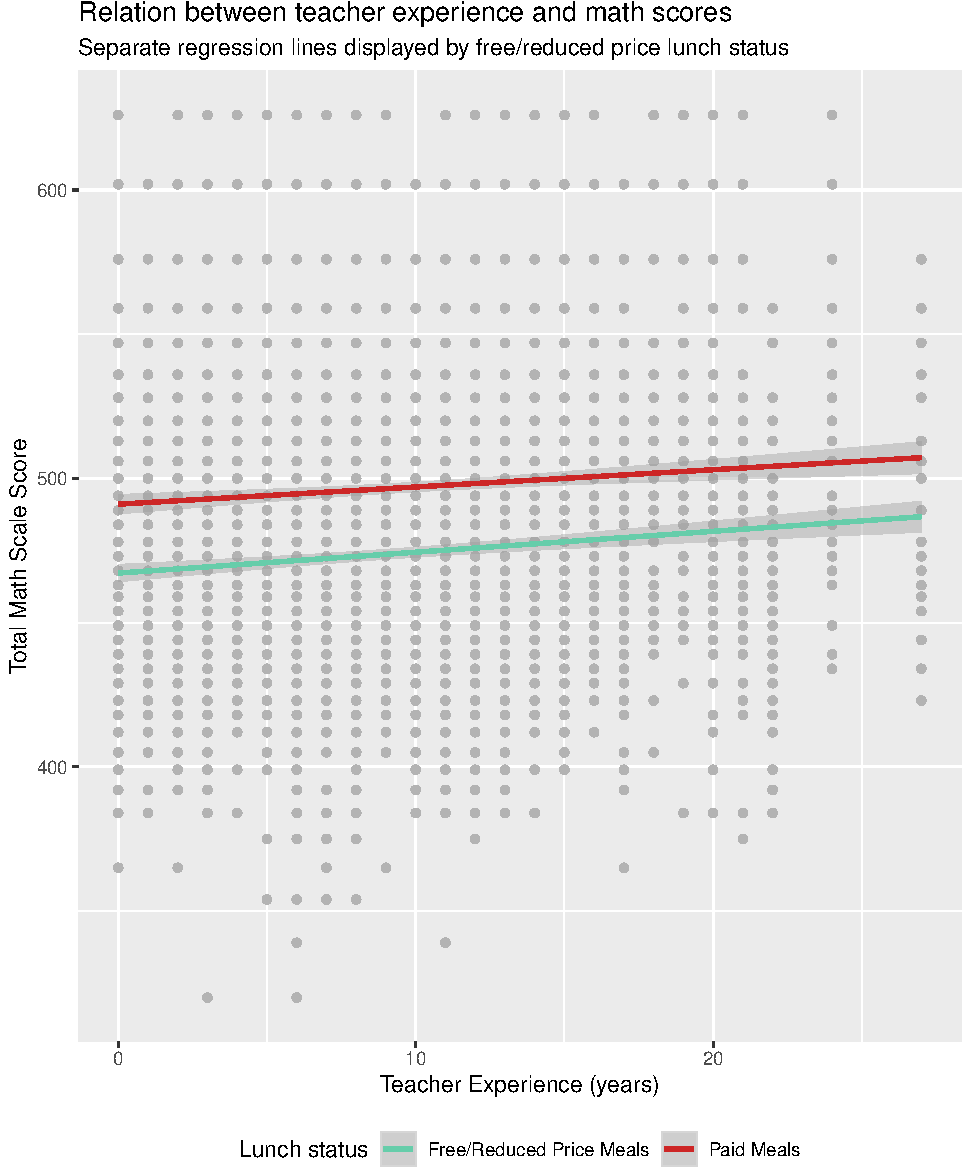
\includegraphics{Lab_8_files/figure-latex/import_data-1.pdf}
\caption{}
\end{figure}

Wehman, Chan, Ditchman, and Kang (2014) conducted a case study to
examine the the effect of supported employment on vocational
rehabilitation outcomes of transition-age youth. Other researchers
examined the exmployability skills for entry-level employees with and
without disabilities ({\textbf{???}}).

\section{Methods}\label{methods}

We report how we determined our sample size, all data exclusions (if
any), all manipulations, and all measures in the study.

\subsection{Participants}\label{participants}

\subsection{Material}\label{material}

\subsection{Procedure}\label{procedure}

\subsection{Data analysis}\label{data-analysis}

We used R (Version 3.6.1; R Core Team, 2019) and the R-packages
\emph{dplyr} (Version 0.8.3; Wickham, François, Henry, \& Müller, 2019),
\emph{forcats} (Version 0.4.0; Wickham, 2019a), \emph{ggplot2} (Version
3.2.1; Wickham, 2016), \emph{here} (Version 0.1; Müller, 2017),
\emph{janitor} (Version 1.2.0; Firke, 2019), \emph{papaja} (Version
0.1.0.9842; Aust \& Barth, 2018), \emph{purrr} (Version 0.3.2; Henry \&
Wickham, 2019), \emph{readr} (Version 1.3.1; Wickham, Hester, \&
Francois, 2018), \emph{rio} (Version 0.5.16; C.-h. Chan, Chan, Leeper,
\& Becker, 2018), \emph{stringr} (Version 1.4.0; Wickham, 2019b),
\emph{tibble} (Version 2.1.3; Müller \& Wickham, 2019), \emph{tidyr}
(Version 1.0.0; Wickham \& Henry, 2019), \emph{tidyverse} (Version
1.2.1; Wickham, 2017), and \emph{tinytex} (Version 0.17; Xie, 2019) for
all our analyses.

\section{Results}\label{results}

Table 1 demonstrates the relationship between teacher experience and
student's math scale scores. The two regression lines demonstrate
differences between free and reduced price lunch status, which students
who are not eligible for free and reduced price lunch scoring, in
general, higher than those who do. In general, it does not appear that
teacher experience significantly impacts this difference, as math scores
for students both with and without free and reduced price lunch status
appears to increase at approximately the same rate.

\section{Discussion}\label{discussion}

\newpage

\section{Table 1}\label{table-1}

\newpage

\section{References}\label{references}

\begingroup
\setlength{\parindent}{-0.5in} \setlength{\leftskip}{0.5in}

\hypertarget{refs}{}
\hypertarget{ref-R-papaja}{}
Aust, F., \& Barth, M. (2018). \emph{papaja: Create APA manuscripts with
R Markdown}. Retrieved from \url{https://github.com/crsh/papaja}

\hypertarget{ref-R-rio}{}
Chan, C.-h., Chan, G. C., Leeper, T. J., \& Becker, J. (2018).
\emph{Rio: A swiss-army knife for data file i/o}.

\hypertarget{ref-R-janitor}{}
Firke, S. (2019). \emph{Janitor: Simple tools for examining and cleaning
dirty data}. Retrieved from
\url{https://CRAN.R-project.org/package=janitor}

\hypertarget{ref-R-purrr}{}
Henry, L., \& Wickham, H. (2019). \emph{Purrr: Functional programming
tools}. Retrieved from \url{https://CRAN.R-project.org/package=purrr}

\hypertarget{ref-R-here}{}
Müller, K. (2017). \emph{Here: A simpler way to find your files}.
Retrieved from \url{https://CRAN.R-project.org/package=here}

\hypertarget{ref-R-tibble}{}
Müller, K., \& Wickham, H. (2019). \emph{Tibble: Simple data frames}.
Retrieved from \url{https://CRAN.R-project.org/package=tibble}

\hypertarget{ref-R-base}{}
R Core Team. (2019). \emph{R: A language and environment for statistical
computing}. Vienna, Austria: R Foundation for Statistical Computing.
Retrieved from \url{https://www.R-project.org/}

\hypertarget{ref-wehman2014}{}
Wehman, P., Chan, F., Ditchman, N., \& Kang, H.-J. (2014). Effect of
supported employment on vocational rehabilitation outcomes of
transition-age youth with intellectual and developmental disabilities: A
case control study. \emph{Intellectual and Developmental Disabilities}.

\hypertarget{ref-R-ggplot2}{}
Wickham, H. (2016). \emph{Ggplot2: Elegant graphics for data analysis}.
Springer-Verlag New York. Retrieved from
\url{https://ggplot2.tidyverse.org}

\hypertarget{ref-R-tidyverse}{}
Wickham, H. (2017). \emph{Tidyverse: Easily install and load the
'tidyverse'}. Retrieved from
\url{https://CRAN.R-project.org/package=tidyverse}

\hypertarget{ref-R-forcats}{}
Wickham, H. (2019a). \emph{Forcats: Tools for working with categorical
variables (factors)}. Retrieved from
\url{https://CRAN.R-project.org/package=forcats}

\hypertarget{ref-R-stringr}{}
Wickham, H. (2019b). \emph{Stringr: Simple, consistent wrappers for
common string operations}. Retrieved from
\url{https://CRAN.R-project.org/package=stringr}

\hypertarget{ref-R-tidyr}{}
Wickham, H., \& Henry, L. (2019). \emph{Tidyr: Easily tidy data with
'spread()' and 'gather()' functions}. Retrieved from
\url{https://CRAN.R-project.org/package=tidyr}

\hypertarget{ref-R-dplyr}{}
Wickham, H., François, R., Henry, L., \& Müller, K. (2019). \emph{Dplyr:
A grammar of data manipulation}. Retrieved from
\url{https://CRAN.R-project.org/package=dplyr}

\hypertarget{ref-R-readr}{}
Wickham, H., Hester, J., \& Francois, R. (2018). \emph{Readr: Read
rectangular text data}. Retrieved from
\url{https://CRAN.R-project.org/package=readr}

\hypertarget{ref-R-tinytex}{}
Xie, Y. (2019). \emph{Tinytex: Helper functions to install and maintain
'tex live', and compile 'latex' documents}. Retrieved from
\url{https://CRAN.R-project.org/package=tinytex}

\endgroup


\end{document}
